\documentclass[a4paper,titlepage]{jreport}
\topmargin -15mm	\textheight 250mm	\textwidth 180mm
\oddsidemargin -10mm	\evensidemargin -10mm

\usepackage[dvips]{graphics}
%\usepackage{geometry}
\usepackage{ascmac}
\usepackage{bm}

\renewcommand{\bibname}{参考文献}

\begin{document} %ドキュメント開始

\title{LAM/MPI マニュアル} %タイトル
\date{\today}
\author{谷 合 由 章\thanks{mail:yosi@bcl.sci.yamaguchi-u.ac.jp}}
\maketitle % タイトル作成

\tableofcontents % 目次

\newpage % 新しいページへ

\part{LAMの説明書}

\chapter{LAM/MPIについて \label{app:LAM}}
MPI(Message Passing Interface)は,メッセージ通信によって並列化
を行う標準規格です.その規格に準拠して作成されたライブラリが
LAM/MPIです.MPIは規格であるので,実際に並列化を行うときLAMの
機能が中心になります.MPIという大前提のものがどういう感じであ
るかを説明し,その後メインのLAM/MPIに関する実戦的なところを説
明します.

\section{MPIについて}

\subsection{MPIの現在までの流れ}
1992年4月29-30日に「分散メモリ環境におけるメッセージ通信のための
標準に関するワークショップ」においてMPIの標準化が始まった.
このワークショップはバージニア州ウィリアムズバーグで「並列コンピューティング
研究センタ」の主催によって開催された.1992年11月に,Dongarra,Hempel,Hey,Walker
により,MPI1として知られる予備的な草案が提示された.それは並列化の論議を促進
するため
のたたき台として役割りを果たした.論議には40を越える団体が参加して,メッセージ
通信のためのライブラリインターフェ−スの標準に関する議論と定義が度々行われて
きた.  現在ではMPI2という標準が設計されるに至っている.

\subsection{どういう目標があったのか}
Message Passing Interface の目標は,メッセージ通信を行うプログラムを
書くための,広く一般に使われる標準を作り出すことのもとに設計された.
この目標を実現するには,MPIは実用的で,ポータブルで,効率がよくかつ融通の
効くメッセージ通信の標準を確立しなければならない.以下に全ての目標のリスト
を以下に示す.

\begin{itemize}
\item アプリケーションプログラムから呼ぶためのインタフェースを設計する.
\item 効率のよい通信を可能にすること.メモリ間コピーを避け,計算と通信
      を並行して進めることができ,通信プロセッサがあれば処理の一部を
      それに任せるようなもの.
\item 異機種環境でも使用できる処理系に備える.
\item C言語やFortran言語のための使い易い呼び出し形式を可能にする.
\item 信頼できる通信インタフェースを想定する.ユーザーは通信障害
      に対処する必要がない.そのような障害は下位の通信サブシステムが
      処理する.
\item PVM,NX,Express,p4などの既存のインタフェースとそれほど違わない
      インタフェースで,なおかつより融通の効く拡張機能を可能にする
      インタフェースを定義する.
\item 多くのベンダのプラットフォーム上に実現でき,その際,下位の通信
      およびソフトウェアに大きな変更を加えずに済むインタフェースを
      定義する.
\item このインタフェースの意味は言語に依存するべきではない.
\item このインタフェースは,マルチスレッド環境への対応が可能なように
      設計するべきである.
\end{itemize}

\subsection{概要}
MPI(Message Passing Interface)は得に分散メモリを備える並列マシンで広く
用いられている.その種類にはいろいろあるが,プロセスがメッセージによって
通信を行うということが基本概念になる.\\

設計においては,既存のメッセージ通信システムが持つもっとも魅力的な機能の
数々を採り入れるように努められた.\\

メッセージ通信の標準を確立する主な利点は,ポータビリティと使いやすさに
にある.分散メモリ環境の中でも得に,高いレイヤ層でのルーチンやアブスト
ラクションが低いレイヤのメッセージ通信ルーチンの上に構築されているもの
では,標準化の利点は明白である.さらに,定義に沿ったルーチンを提供している.
このようなルーチン群があれば,ベンダは,それが効率よく実現したり,あるいは
場合によってはそれ専用のハードウェアを用意したりすることができ,それに
よりスケ−ラビリティを高めることができる.

\begin{itemize}
\item[] MPI2標準に含まれるもの
\item 1対1通信(MPI1)
\item 集団操作(MPI1)
\item プロセスグループ(MPI1)
\item 通信コンテキスト(MPI1)
\item プロセストポロジー(MPI1)
\item Fortran77言語とC言語の呼び出し形式(MPI1)
\item 環境管理と問い合わせ(MPI1)
\item プロファイリングインタフェース(MPI1)
\item 入出力(I/O)(MPI2)
\item Fortran90,C++言語向けの枠組み(MPI2)
\item 動的プロセス制御(MPI2)
\item 片側通信(MPI2)
\item グラフィックス(MPI2)
\item 実時間対応(MPI2)
\end{itemize}

\section{LAM/MPI}
実際にプログラムするときにMPIの機能を提供するのはLAM/MPIである.
LAM(Local Area Multicomputer)は,ノートルダム大学の科学コンピュータ
研究室(Laboratory for Scientific Computing,University of Nortre
 Dame)が作成したフリーのMPIライブラリである.現在はインディアナ大学
(Indiana university)によって引き継がれ,大幅にバージョンアップが行
われている.機能的に
も高いものになってきており,今後も発展が見込まれる.

\subsection{LAM/MPI のサポート}
LAMユーザガイドの29ページ

LAM7.0.3では全てのMPI-1関数をサポートしている.MPI-2は
大体サポートされているが一部未サポートがある.

\subsection{LAM/MPIについて(実践)}
LAM/MPIのプログラムが書けるとしても,それだけではプログラム
は動かない.LAM/MPIを構築することに関する管理者向けのものは
付録\ref{app:kanri}に,コンパイルや実行についてのユーザ向けのも
のは付録\ref{app:user}を参照してください.

\chapter{並列計算環境の構築(管理者向け)\label{app:kanri}}
以下の設定環境は VINE LINUX 2.6 CR で行いました.
LAM パッケージを利用する場合,パスワードなしでログインできる
設定を行っておく必要があります.ssh か rsh のいずれか1つを
使う環境に合わせて選択し,その設定を行ってください.

1000 Base のGiga Bit Ethernet の設定と Intel製のコンパイラ
の使用はオプションとしてあります.これらを採りいれなくても,
MPIパッケージは使用できるのですが,MPIによる並列計算のパフォ
ーマンスをより上げる意味で行いました.

以上のことが終われば, LAM を利用できることになります.

\section{パスワードなしでのログイン}

\subsection{rsh, rlogin編}

\subsubsection{【はじめに】}
rsh, rloginは他のホストにネットワークを経由してログイン
を可能にします.ですが, ネットワークの経路上は暗号化され
ないため, セキュリティ上非常に危険にさらされることになります.

しかし, 経路がインターネットなどの不特定多数の経路(人)がいな
いローカルネットワークではそうではありません. 暗号化すること
に比べて, 非常にめんどうな鍵の管理を考えなくてすみます. さら
に, 暗号化と復号化にかかるコストもなくなります(しかし, 通信
が遅い場合や通信内容が重い場合, sshには圧縮機能があるため, 有
効利用できます).

並列計算環境を作る上でrsh, rloginの有用性を持っていますので, ここに
文章としてまとめています.

\subsubsection{【パスワードなしでログインできるまで】}

ここでは, 見通しとして概要を見ます.

\begin{description}
\item[1.] rsh, loginのサービスを有効にする.
\item[2.] pam認証において, パスワードを必要なしにする.
\item[3.] 設定を反映させるために, inetを再起動する.
\item[4.] /etc/hosts.equivやユーザのホームディレクトリ\~/.rhostsに
          ログインを許可するホスト, ユーザを書いておく.
\end{description}

\subsubsection{【詳細な設定】}
\subsubsection{[pam認証でホスト間認証を設定する]}

          pam認証は, さまざまなアプリケーションの認証を共通に扱う
          ものです. プログラマは, パスワードの要求, 判定などを, pam
          の共有ライブラリにまかせることができます. そして, 柔軟な認証
          設定ができ, 強力な認証機能をもっています.

          具体的にrsh, rloginでの認証をパスワードなしにする設定を以下行って
          いきます. 

\begin{description}
\item[1.] rshでの設定

/etc/pam.d/rshにrshの設定ファイルがおいてあります. 以下にその中身を載せました.

\newpage

\begin{quote}
\begin{screen}
\begin{verbatim}
#%PAM-1.0
auth       required	/lib/security/pam_nologin.so
#auth       required	/lib/security/pam_securetty.so
auth       required     /lib/security/pam_env.so
auth        required    /lib/security/pam_rhosts_auth.so \
  hosts_equiv_rootok promiscuous
account    required	/lib/security/pam_stack.so service=system-auth
session    required	/lib/security/pam_stack.so service=system-auth
\end{verbatim}
\end{screen}
\end{quote}

pam\_rhosts\_auth.so の hosts\_equiv\_rootok promiscuousはrootでのログインを
可能にするオプションです.これを設定するのはセキュリティ上, 非常に危険です.

\item[2.] rloginでの設定

/etc/pam.d/rlogin にrloginの設定ファイルがおいてあります. 以下にその
中身を載せました.

\begin{quote}
\begin{screen}
\begin{verbatim}
#%PAM-1.0
auth       required	/lib/security/pam_nologin.so
#auth       required	/lib/security/pam_securetty.so
auth       required     /lib/security/pam_env.so
#auth       sufficient	/lib/security/pam_rhosts_auth.so
#auth       required	/lib/security/pam_stack.so service=system-auth
auth       required     /lib/security/pam_rhosts_auth.so\
 hosts_equiv_rootok promiscuous
account    required	/lib/security/pam_stack.so service=system-auth
password   required	/lib/security/pam_stack.so service=system-auth
session    required	/lib/security/pam_stack.so service=system-auth
\end{verbatim}
\end{screen}
\end{quote}

pam\_rhosts\_auth.so の hosts\_equiv\_rootok promiscuousはrootでのログインを
可能にするオプションです.これを設定するのはセキュリティ上, 非常に危険です.

\end{description}

\subsubsection{[パスワードなしでログインできるホストを決める]}

          rsh, rloginのサービスを提供して, パスワードなしのログインが
          できるようになったのですが, それでめでたしめでたしとはいきません.
          誰でもパスワードなしで, どこからでもログインできることは危険きわまり
          ないです. そこで, ここでは特定のホストだけにパスワードなしでのロ
          グインを許可するように設定を行います.\\

          設定には2通りあり, 1つはユーザ個人で許可を許せるユーザレベルでの
          設定, もう1つは管理者によって許可するホストレベルでの設定です.
          以下, この2つについて, それぞれの設定を行います.

\newpage

\begin{description}
\item[1.] ユーザレベルでの許可をする

          設定ファイルはホームディレクトリの\~/.rhostsにおきます.
          このファイルに書かれているホストに対して許可を出します. 
          書いていないホストはログインすることはできません.\\

          書式は, 箇条書で, ホスト名, FQDN, IP addressのいずれでも
          OKです. ただし, それによって名前解決ができることが必須条件
          です.\\
          
          なお, ホストの横に1つスペースをおいて, ユーザ名を書いておくと
          そのホストのそのユーザのみの許可だけを許すことができます.

          以下, その例を載せます.

\begin{quote}
\begin{screen}
\begin{verbatim}
[例] 
node1.sample.ac.jp user1
node2.sample.ac.jp
\end{verbatim}
\end{screen}
\end{quote}

          上の例では, node1からはユーザuser1だけがログイン可能なことが
          わかります. 1つ下のnode2からは, どのユーザでも(rootはpam認証
          の設定次第で)ログインできることになります.\\

          ファイルがない場合は作成してください. 作成した場合, ファイルアクセスの
          パーミッションを「chmod 600 .rhosts」を実行し, 変えておく
          必要があります.
          万が一, ファイルのパーミッションの設定で, 他人がそのファイル
          に任意のコードを書き込めた場合, ログインなどの際に.rhostsが読み込まれ
          意図しない動作を行ったり, システムを乗っ取られたりする可能性
          があります.

\item[2.] ホストレベルでの許可

          /etc/hosts.equivが設定ファイルです. ホストレベルでの認証の場合にこ
          れを記述する.書式は「~/.rhosts」と同様である.

\end{description}

\subsection{ssh編}

\subsubsection{【設定の概要】}

毎回ログインする際にパスワードの入力がありますが, それを行
わないでログインすることもできます.  SSH1プロトコルではRhostsRSA認
証, SSH2ではホストベース認証がそれに当たります. その他ssh-agentを利用す
る方法もありますが, ここでは SSH2のホストベース認証を扱います.
以下の作業は\cite{ssh}やLAMの公式ページのFAQを参考にしています.

\subsubsection{【ホストベース認証】}
ホストベース認証は, パスワードの入力なしにログインすることができることを
前述しました. これには2つのレベル, クライアントレベルとホストレベルでの
管理ができます.

クライアントレベルでの認証は管理者でなくても, 自由にパスワードを入力なし
でログインすることを設定することができます.   ホストレベルでは, 管理者の
みがパスワードの入力なしにするホストを決めることができます. 

\subsubsection{【サポート】}
Hostbased認証がサポートされているのは OpenSSH-2.9以降のバージョン
みたいです. 詳しくは公式ホームページなどを参照してください.

\subsubsection{【バグフィックス】}
「openssh-3.5p1」に不都合があるようです. これによってホストベース認証ができない
ことがわかっています.そのため, Vine2.6の初期のバグを含んだsshパッケージ
を「openssh-3.5p2」にする必要があります.なお, 本研究室では, aptでアップグ
レード可能なようにしています.\\

[訂正]

実際のところバグはないような気がします.  詳しくはわかりませんの
で, 御本人でお確かめください.

\subsubsection{【手順】}

Hostbased認証を行う上で, おおまかな作業手順です.

\begin{enumerate}
\item サーバでホストベース認証ができるようにする.(ファイル/etc/ssh/sshd\_confの設定)

\item クライアントのホスト鍵をサーバのファイル /etc/ssh/ssh\_known\_hosts2に登録する.

\item サーバのファイル /etc/ssh/shosts.equiv を正しく設定しておく.
\end{enumerate}

\subsubsection{【設定が必要なファイル】}
見通しが良くなるように, どのファイルを変更することになるのかを
上げました.

\begin{enumerate}
\item /etc/shosts.equiv

          パスワードなしでログインを許すホストを決める設定ファイルです.
          書くときはホストを特定する名前(IP, FQDN, ホスト名) を使います.
          箇条書をした各々のホストの横1つスペースをおいてユーザ名を書
          くことで, ユーザレベルでのログインを制限できます.

\item /etc/ssh/sshd\_config

          SSHサーバの設定ファイルです. ホストベース認証を
          行うように設定変更します. 

\item /etc/ssh/ssh\_known\_hosts2

          /etc/shosts.equivで箇条書したホストの公開鍵を登録しておく
          ファイルです.
          ファイル名の最後に「2」がついていることで, SSH2の場合に参照
          されることになります.
          SSH1の場合はファイル /etc/ssh/ssh\_known\_hosts になります.

\item /etc/ssh/ssh\_host\_dsa\_key と /etc/ssh/ssh\_host\_dsa\_key.pub

          そのホスト自身の公開鍵と秘密鍵を置いておくファイルです.
          二つのファイルの名前の違いは最後の「.pub」の拡張子で
          ,ついているものが公開(public)鍵です.
          ほとんどの場合, インストールされたときに作成されています. 
          この二つのファイル(鍵)の作成は, コマンドラインで行います.

\end{enumerate}

\subsubsection{【arisサーバでの具体的な設定】}

aris並列計算機サ−バから, 実際に計算するホストにホストベース認証できる
ように設定します(クライアントの設定). 逆に, 計算ホストからサーバへの
認証には, パスワード認証, DSA認証を使い, パスワードの入力を必要に
します.

\subsubsection{[クライアントの設定]}

ファイル \~/.ssh/configを作成しておく.

\begin{quote}
\begin{screen}
\begin{verbatim}
 Host *
   ForwardAgent no
   ForwardX11 no
   PreferredAuthentications hostbased,pubkey,password # 優先する認証の順番
   PubkeyAuthentication yes # 公開鍵認証(SSH2)
   RhostsAuthentication no # 普通は no
   RhostsRSAAuthentication no # 普通は no
   RSAAuthentication yes # 公開鍵認証(SSH1)
   PasswordAuthentication yes # パスワード認証
   HostbasedAuthentication yes # ホストベース認証
   BatchMode no
   CheckHostIP yes
   StrictHostKeyChecking ask
   IdentityFile ~/.ssh/identity
   IdentityFile ~/.ssh/id_rsa
   IdentityFile ~/.ssh/id_dsa
   Port 22
   Protocol 2,1 # 利用するプロトコルバージョン
   Cipher 3des # ssh1で使う暗号化方式(blowfish も可)
   Ciphers aes128-cbc,3des-cbc,blowfish-cbc,cast128-cbc,arcfour,aes192-cbc,aes256-cbc # SSH2
   EscapeChar ~
Host *
	ForwardX11 yes
\end{verbatim}
\end{screen}
\end{quote}

PrefferedAuthentication の項目は, 認証の際に優先して行う認証方法を
スペースをいれずに書きます. 上では, ホストベース認証, 公開鍵認証, パスワード
認証の順になります.

\subsubsection{[サーバの設定]}

\begin{enumerate}
\item 公開鍵, 秘密鍵を作成する

\begin{quote}
\begin{screen}
\begin{verbatim}
$ssh-keygen -t dsa -f /etc/ssh/ssh_host_dsa_key -N ""
\end{verbatim}
\end{screen}
\end{quote}

      これで公開鍵, 秘密鍵が作成されます. 作成されている場合は,
      作成しなくてもよいです. ユーザレベルでの公開鍵, 秘密鍵は
      パスフレーズで暗号化されておかれるのですが, このホスト鍵は
      暗号化してはいけません. 暗号化しないために指定したオプション
      が「$-N\hspace{3mm} ""$」になります.

\item /etc/ssh/sshd\_config

\begin{quote}
\begin{screen}
\begin{verbatim}
Port 22
Protocol 2 # SSH2のみでの認証
#ListenAddress 0.0.0.0
#ListenAddress ::

# HostKey for protocol version 1
#HostKey /etc/ssh/ssh_host_key
# HostKeys for protocol version 2
#HostKey /etc/ssh/ssh_host_rsa_key
HostKey /etc/ssh/ssh_host_dsa_key # ホスト鍵にdsaを使う

# Lifetime and size of ephemeral version 1 server key
#KeyRegenerationInterval 3600
#ServerKeyBits 768

# Logging
#obsoletes QuietMode and FascistLogging
#SyslogFacility AUTH
SyslogFacility AUTHPRIV
#LogLevel INFO

# Authentication:

#LoginGraceTime 120
#PermitRootLogin yes
PermitRootLogin no
#StrictModes yes

#RSAAuthentication yes 
PubkeyAuthentication yes # SSH2で公開鍵認証を使う
#AuthorizedKeysFile	.ssh/authorized_keys

# rhosts authentication should not be used
RhostsAuthentication no # 普通 no
# Don't read the user's ~/.rhosts and ~/.shosts files
IgnoreRhosts no # ユーザレベルでのホストベース認証を禁止
# For this to work you will also need host keys in /etc/ssh/ssh_known_hosts
RhostsRSAAuthentication no # 普通 no
# similar for protocol version 2
HostbasedAuthentication no # ホストベース認証を使わない
# Change to yes if you don't trust ~/.ssh/known_hosts for
# RhostsRSAAuthentication and HostbasedAuthentication
IgnoreUserKnownHosts yes

# To disable tunneled clear text passwords, change to no here!
PasswordAuthentication yes # パスワード認証を使う
PermitEmptyPasswords no 

# Change to no to disable s/key passwords
#ChallengeResponseAuthentication yes
\end{verbatim}
\end{screen}
\end{quote}

\begin{quote}
\begin{screen}
\begin{verbatim}
# 前ページの続き
#
# Kerberos options
#KerberosAuthentication no
#KerberosOrLocalPasswd yes
#KerberosTicketCleanup yes

#AFSTokenPassing no

# Kerberos TGT Passing only works with the AFS kaserver
#KerberosTgtPassing no

# Set this to 'yes' to enable PAM keyboard-interactive authentication 
# Warning: enabling this may bypass the setting of 'PasswordAuthentication'
#PAMAuthenticationViaKbdInt no

#X11Forwarding no
X11Forwarding yes
#X11DisplayOffset 10
#X11UseLocalhost yes
#PrintMotd yes
#PrintLastLog yes
#KeepAlive yes
#UseLogin no
UsePrivilegeSeparation no # ホストベース認証を使う場合, yes
#PermitUserEnvironment no
#Compression yes

#MaxStartups 10
# no default banner path
#Banner /some/path
#VerifyReverseMapping no

# override default of no subsystems
Subsystem	sftp	/usr/libexec/openssh/sftp-server
\end{verbatim}
\end{screen}
\end{quote}

\end{enumerate}

\subsubsection{【並列計算におけるクライアントの設定】}

\subsubsection{[公開鍵, 秘密鍵を作成する]}

\begin{quote}
\begin{screen}
\begin{verbatim}
$ ssh-keygen -t dsa -f /etc/ssh/ssh_host_dsa_key -N ""
\end{verbatim}
\end{screen}
\end{quote}

\subsubsection{[/etc/shosts.equiv]}

一行ごとにホストを書きます.

\begin{quote}
\begin{screen}
\begin{verbatim}
node1.sample.ac.jp
111.111.111.111 user1
node2
\end{verbatim}
\end{screen}
\end{quote}

上の例では

\begin{enumerate}
\item node1.sample.ac.jpからの接続を許可.
\item 111.111.111.111からユーザuser1のみのログインを許可.
\item ホストnode2からの接続を許可.
\end{enumerate}

という設定になります.

\subsubsection{[/etc/ssh/ssh\_known\_hosts2]}

ホストベース認証を許可するホストの公開鍵を置くファイルです.

\begin{quote}
\begin{screen}
\begin{verbatim}
$ cat <公開鍵ファイル> >> /etc/ssh/ssh_known_hosts2
\end{verbatim}
\end{screen}
\end{quote}

を実行して追加してください. cp などによってファイルを上書きしないように注意してください. 

\begin{quote}
\begin{screen}
\begin{verbatim}
ssh-dss AAAAB3NzaC1kc3MAAACBAJ4gcPqz2A4X4yDUfnlgFNgCMrbzALlTd9l4doGYJrDCYD
oOwgUkRrmf14yeQKct9SSXPGVsc88N6a6eRwKBWGrm7MGaTNMwllY+w0eDIaFXgbFXGqx1pnz4
esiffS5f9ap3/pVXXaoCTSGXg/wN8hqaG58OY8bySTX6HK3JWTZ1AAAAFQCzcweCvbIyLJqidT
inGYradMb/CwAAAIBMF2k+acHAAn+md51WUWru2p+e4jV7+SwyS7wdh2lwhfB81qOdGvP8BgY9
DceK5P3srrnC6ZlUt67IyuKD6VxsUce8L8XELsHlRYoE0+w+WaPnaXAzxMisPFZGpClGnzsutN
RSUMNq15xszztqHQAhXX2dE/iAAf94W8qi5BDqbAAAAIAveEucknapYS2VUtuck7qyT21DuVdZ
jgEqVXlWHFxr06mrdWq7Hp3lRXF6++WYmK/QWUR8BjngXQ1PFCYW9JAiyQIWFBrWfWtbElmR6g
r/qXZOsNXNjoDxdDG5SwXMyJbhJaf3aXK7YGvq9FKSCEoNjadQ19VITmw6C8dYFNh8yQ=
\end{verbatim}
\end{screen}
\end{quote}
追加した公開鍵が上のように ssh-dss の前にホスト名などが記入されていない場合, editor で
ホスト名, IP address, FQDNを以下のように記入してください.

\begin{quote}
\begin{screen}
\begin{verbatim}
node2, node2.sample.ac.jp,222.222.222.222 ssh-dss AAAAB3NzaC1kc3
MAAACBAJ4gcPqz2A4X4yDUfnlgFNgCMrbzALlTd9l4doGYJrDCYDoOwgUkRrmf14yeQKct9SSX
PGVsc88N6a6eRwKBWGrm7MGaTNMwllY+w0eDIaFXgbFXGqx1pnz4esiffS5f9ap3/pVXXaoCTS
GXg/wN8hqaG58OY8bySTX6HK3JWTZ1AAAAFQCzcweCvbIyLJqidT inGYradMb/CwAAAIBMF2k
+acHAAn+md51WUWru2p+e4jV7+SwyS7wdh2lwhfB81qOdGvP8BgY9DceK5P3srrnC6ZlUt67Iy
uKD6VxsUce8L8XELsHlRYoE0+w+WaPnaXAzxMisPFZGpClGnzsutNRSUMNq15xszztqHQAhXX2
dE/iAAf94W8qi5BDqbAAAAIAveEucknapYS2VUtuck7qyT21DuVdZjgEqVXlWHFxr06mrdWq7H
p3lRXF6++WYmK/QWUR8BjngXQ1PFCYW9JAiyQIWFBrWfWtbElmR6gr/qXZOsNXNjoDxdDG5SwX
MyJbhJaf3aXK7YGvq9FKSCEoNjadQ19VITmw6C8dYFNh8yQ=
\end{verbatim}
\end{screen}
\end{quote}

\subsubsection{[/etc/ssh/sshd\_config]}

ホストベース認証を許すように設定します.

\begin{quote}
\begin{screen}
\begin{verbatim}
Port 22
Protocol 2,1
#ListenAddress 0.0.0.0
#ListenAddress ::

# HostKey for protocol version 1
HostKey /etc/ssh/ssh_host_key
# HostKeys for protocol version 2
HostKey /etc/ssh/ssh_host_rsa_key
HostKey /etc/ssh/ssh_host_dsa_key

# Lifetime and size of ephemeral version 1 server key
#KeyRegenerationInterval 3600
#ServerKeyBits 768

# Logging
#obsoletes QuietMode and FascistLogging
#SyslogFacility AUTH
SyslogFacility AUTHPRIV
#LogLevel INFO

# Authentication:

#LoginGraceTime 600
#PermitRootLogin yes
PermitRootLogin no
#StrictModes yes

RSAAuthentication yes
PubkeyAuthentication yes
#AuthorizedKeysFile	.ssh/authorized_keys

# rhosts authentication should not be used
RhostsAuthentication no
# Don't read the user's ~/.rhosts and ~/.shosts files
IgnoreRhosts yes # ユーザレベルでのホストベース認証をさせない
# For this to work you will also need host keys in /etc/ssh/ssh_known_hosts
RhostsRSAAuthentication no
# similar for protocol version 2
HostbasedAuthentication yes # ホストベース認証を許可する
# Change to yes if you don't trust ~/.ssh/known_hosts for
# RhostsRSAAuthentication and HostbasedAuthentication
IgnoreUserKnownHosts yes # ユーザレベルでのホストベース認証をさせない
\end{verbatim}
\end{screen}
\end{quote}

\newpage

\begin{quote}
\begin{screen}
\begin{verbatim}

# To disable tunneled clear text passwords, change to no here!
PasswordAuthentication yes
PermitEmptyPasswords no

# Change to no to disable s/key passwords
#ChallengeResponseAuthentication yes

# Kerberos options
#KerberosAuthentication no
#KerberosOrLocalPasswd yes
#KerberosTicketCleanup yes

#AFSTokenPassing no

# Kerberos TGT Passing only works with the AFS kaserver
#KerberosTgtPassing no

# Set this to 'yes' to enable PAM keyboard-interactive authentication 
# Warning: enabling this may bypass the setting of 'PasswordAuthentication'
#PAMAuthenticationViaKbdInt yes

#X11Forwarding no
X11Forwarding yes
#X11DisplayOffset 10
#X11UseLocalhost yes
#PrintMotd yes
#PrintLastLog yes
#KeepAlive yes
#UseLogin no
UsePrivilegeSeparation yes # ホストベース認証をするときは必要
#Compression yes

#MaxStartups 10
# no default banner path
#Banner /some/path
#VerifyReverseMapping no

# override default of no subsystems
Subsystem	sftp	/usr/libexec/openssh/sftp-server
\end{verbatim}
\end{screen}
\end{quote}

\subsubsection{【再起動】}
サーバ, クライアントのsshdサーバを再起動します. 以上で設定完了です.

\subsubsection{【管理者向け】}
初期設定ファイル \~/.bashrc においては, あらかじめ /etc/skel に対して反映させておくと,
ユーザを追加する度に毎回設定をしなくてすみます.

\subsubsection{【トラブルシューティング】}
以上のことを行っても上手くいかない場合, コマンド /usr/bin/ssh の
ユーザ権限が「s」になっているか確かめてください. なっていない場合, 
以下のコマンドを実行してください.

\begin{quote}
\begin{screen}
\begin{verbatim}
$ chmod u+s /usr/bin/ssh
\end{verbatim}
\end{screen}
\end{quote}

\section{LAMのインストール}

\section{Gigabit Network の設定}

\subsection{はじめに}
研究室に GigaBit 環境を取りいれるための設定です。
最低今までの3倍(?)の速度がでて、よりよい環境でコンピュータを
扱えると思います.

1000MBでの通信をする場合、それに対応したNIC(LAMカード)が
必要になります。そして、NICを使うためのドライバーをインス
トールする必要があります。

\subsection{作業手順}

以下は作業手順と方法です。行う作業としては4つの項目が
あります。

\subsubsection{【kernel のインストール】}

\begin{enumerate}
\item rootになる.
\item ディレクトリ /home/public/Kernel\_Gigabit/ に移動する.
\item kernelをインストールする.
\end{enumerate}

\subsubsection{【LILO の設定】}

\begin{enumerate}
\item rootになる.
\item エディタでファイル /etc/lilo.conf を開く.
\item エディタで開いたら、下のような感じの内容がでてきます。
        以下のように変更してください。
\end{enumerate}

\begin{quote}
\begin{screen}
\begin{verbatim}
「変更1」

prompt
timeout=50
default=linux
boot=/dev/hda
map=/boot/map
install=/boot/boot.b
message=/boot/message
linear

image=/boot/vmlinuz-2.4.19-0vl11    <------ コピー(この行から)
        label=linux
        read-only
        root=/dev/hda2              <------ コピー(この行まで)

\end{verbatim}
\end{screen}
\end{quote}

\begin{quote}
\begin{screen}
\begin{verbatim}
「変更2」

prompt
timeout=50
default=linux
boot=/dev/hda
map=/boot/map
install=/boot/boot.b
message=/boot/message
linear

image=/boot/vmlinuz-2.4.19-0vl11    
        label=linux
        read-only
        root=/dev/hda2

image=/boot/vmlinuz-2.4.19-0vl11    <---- 張り付けた(始
        label=linux
        read-only
        root=/dev/hda2              <---- 張り付けた(終
\end{verbatim}
\end{screen}
\end{quote}

\begin{quote}
\begin{screen}
\begin{verbatim}
「変更3」

prompt
timeout=50
default=linux
boot=/dev/hda
map=/boot/map
install=/boot/boot.b
message=/boot/message
linear

image=/boot/vmlinuz-2.4.19-0vl11    
        label=linux-old             <---- 変更した。
        read-only
        root=/dev/hda2

image=/boot/vmlinuz                 <---- 変更した。   
        label=linux
        read-only
        root=/dev/hda2              
\end{verbatim}
\end{screen}
\end{quote}

コマンド /sbin/lilo を実行してください. もしファイ
ル /etc/lilo.conf の設定がおかしい場合, errorメッセ
ージがでますので, もう一度確認してみてください.

\subsubsection{【NIC(LAMボード)をつける】}

\begin{enumerate}
\item まずコンピュータを停止する.
\item システムが停止した状態を確認して電源コンセントを抜く。
\item コンピュータにNICをつける。(静電気に注意。作業をする前になに
      か金属に触れておくなどする)
\item 電源コンセントを入れ、コンピュータを起動する。
\end{enumerate}

\subsubsection{【netcfgで設定】}

\begin{enumerate}
\item 電源コンセントを入れ, コンピュータを起動する.
\item 新しいカーネルを選択する.
\item rootでログインする.
\item コマンド dmesg を実行して、eth1かeth0かを調べる.
\item コマンド netcfg を実行し、インタフェースのタブを押す.
\item 先ほど調べたethに関して無い場合は追加, ある場合はそれの変更をする.
\item 追加や変更内容は以前使っていた設定と同じにする.
\item 設定を保存して、終了する。
\item コマンド「/etc/init.d/network restart」を実行する.
\end{enumerate}

\subsection{終わりに}

以上で設定は終了となります.なにかおかしなことになったり、よくわから
ない点があれば聞いてください。あらかじめ言ってもらえれば、この作業を
しますので、連絡してください。おかしい点があれば、教えてください。

\section{Intel Compilerの設定}

\subsection{まえがき}
LAMは, デフォルトで gcc コンパイラを使います.gcc より実行速
度の早くなるコンパイラにIntel製のコンパイラをインストールします.

\subsection{変更するメリット}

      Intel製のコンパイラは gcc に比べて2〜4割の実行時間の短縮を見込めます. 

\subsection{gcc から Intel製のコンパイラへ}

\subsubsection{インストール}

\begin{enumerate}
\item ディレクトリ /home/public/MPI/Intel\_Compiler/ にあるファイル intel\_
      compiler.tgz をひろってくる.

\item コマンド \$ su - でrootになる.

\item ファイル intel\_compiler.tgz を展開して ./install を実行。

\item is32のコンパイラを選ぶ(ライセンスに関しては、全て「accept」で良い)

\item インストールディレクトリはdefault(/opt)で良い。(/usr/localなども可)

\end{enumerate}

\subsection{管理者向け}
初期設定ファイル \~/.bashrc においては, あらかじめ /etc/skel に対
して反映させておくと, ユーザを追加する度に毎回設定をしなくてすみます.

\chapter{操作方法(ユーザ向け)\label{app:user}}

\section{研究室内編}

\subsection{最初にしておく設定}
LAMでSSH, Intel Compilerを利用するための設定を
行っておく必要があります. LAMは, インストール
した時点で rsh と gcc を使って並列計算すること
ができます. rsh はセキュリティを考えるとできる
だけ使用したくありません. gcc より実行速度の早
くなるコンパイラを利用したい. これらのことから
 rsh を ssh に, gcc を Intel製のコンパイラに変
更します.

\subsubsection{【変更するメリット】}

\begin{itemize}
\item SSHの利用

      ssh は秘密鍵, 公開鍵を使って通信内容の暗号化,
      なりすまし対策を行えます.

\item Intel製コンパイラの利用

      Intel製のコンパイラは gcc に比べて2〜4割の実行時間の短縮を見込めます. 

\end{itemize}

\subsubsection{【設定の変更】}

\subsubsection{[rsh から ssh へ]}
          ファイル \~/.bashrc に以下の行をを追加
          してください.  

\begin{quote}
\begin{screen}
\begin{verbatim}
LAMRSH="ssh -x"
export LAMRSH
\end{verbatim}
\end{screen}
\end{quote}
コマンド \$ source \~/.bashrc を実行して, 設定を反映させてください.

\subsubsection{[gcc から Intel製のコンパイラへ]}

\subsubsection{PATH の設定}

          インストールしたら, ディレクトリ /opt 下に配置されているので, PATH
          を追加します. ファイル \~/.bashrc に以下の項目を追加してください.

\begin{quote}
\begin{screen}
\begin{verbatim}
PATH=$PATH:/opt/intel/compiler70/ia32/bin
export PATH
\end{verbatim}
\end{screen}
\end{quote}

          これでIntel製のコンパイラを利用できるようになりました.
          次にLAMでIntel製のコンパイラを使えるようにします. 
          ホームディレクトリ\~/.bashrcに同様に以下の行を加えてください.
\begin{quote}
\begin{screen}
\begin{verbatim}
LAMHCC=icc
export LAMHCC
\end{verbatim}
\end{screen}
\end{quote}
コマンド\$ source \~/.bashrcを実行して, 設定を反映させてください.

\subsection{手順}

流れとしては以下のようになります.

\begin{enumerate}
\item 並列計算させるコンピュータを決める.

\item プログラムを実行できるようにする(LAMの起動).

\item プログラムを実行する.

\item 並列計算を終える.

\end{enumerate}

あらかじめプログラムをコンパイルし,実行ファイルが必要になります(参照)

\subsection{設定, 操作方法}

\subsubsection{【並列計算させるコンピュータを決める】}
計算させるホストを箇条書にします. 
以下のようにファイル \~/lamhosts を作成してください.

\begin{quote}
\begin{screen}
\begin{verbatim}
node1.sample.ac.jp
node2.sample.ac.jp
node3.sample.ac.jp
node4.sample.ac.jp
\end{verbatim}
\end{screen}
\end{quote}

このようにファイル \~/lamhosts に載せたホストは並列計算する
候補でしかありません. というのは, プログラムを実行するとき, オ
プションを指定することで, 候補のうちから選択して計算を行うこと
ができ,資源(CPU,メモリなど)を全て使用しなくてよいです.

\subsubsection{【プログラムを実行できるようにする(LAMの起動)】}
次にコマンド \$ lambootによってLAMの起動を行います. オプショ
ン「-v」は, スタート開始時のプロセスの報告をさせます.

\begin{quote}
\begin{screen}
\begin{verbatim}
$ lamboot -v lamhosts 

LAM 7.0.3/MPI 2 C++/ROMIO - Indiana University

n0<23808> ssi:boot:base:linear: booting n0 (node1.sample.ac.jp)
n0<23808> ssi:boot:base:linear: booting n1 (node2.sample.ac.jp)
n0<23808> ssi:boot:base:linear: booting n2 (node3.sample.ac.jp)
n0<23808> ssi:boot:base:linear: booting n3 (node4.sample.ac.jp)
n0<23808> ssi:boot:base:linear: finished
$
\end{verbatim}
\end{screen}
\end{quote}

上の例の最後に「finished」という出力があることで成功した
ことがわかります.

\subsubsection{【プログラムを実行する】}
実行するにはコマンド \$ mpirun を使います. 以下は, ファイ
ル\~/lamhostsで指定したホスト全てで計算を行います.

\begin{quote}
\begin{screen}
\begin{verbatim}
$ mpirun N <object file>
\end{verbatim}
\end{screen}
\end{quote}

オプション「N」 は全てのホストを示しています.\\

以下のように特定のホスト(n0とn1とn4)を選択することも可能です.

\begin{quote}
\begin{screen}
\begin{verbatim}
$ mpirun n0,1,4 <object file>
\end{verbatim}
\end{screen}
\end{quote}

並列計算を行わせるホスト全てに実行ファイルをおいておく必要
があります. あらかじめ, scpなどでホームディレクトリにおいて
おいてください. しかし, 以下のようにオプション「-s h」を指定
することで, 実行ファイルを並列計算するホストに転送して実行す
ることができます.

\begin{quote}
\begin{screen}
\begin{verbatim}
$ mpirun n1,3 -s h <object file>
\end{verbatim}
\end{screen}
\end{quote}

\subsubsection{【並列計算を終える】}
並列計算(LAM)を終えるとき,以下のコマンドを実行してください.

\begin{quote}
\begin{screen}
\begin{verbatim}
$ lamhalt
\end{verbatim}
\end{screen}
\end{quote}

コマンド lamhalt で正常に終了できなかった(エラーがでた)場合,
以下のコマンドで終了させてください.

\begin{quote}
\begin{screen}
\begin{verbatim}
$ wipe -v ~/lamhosts
\end{verbatim}
\end{screen}
\end{quote}

\newpage

\section{情報演習室編}

\subsection{最初にしておく設定}

以下の作業は www.info.sci.yamaguchi-u.ac.jp, alpha.info.sci.yama
guchi-u.ac.jp, is00.sci.yamaguchi-u.ac.jp のいずれかで行ってくだ
さい.

\subsubsection{【ディレクトリ bin の作成と PATH の設定】}
自分のホームディレクトリに bin というディレクトリを作成してください.

\begin{quote}
\begin{screen}
\begin{verbatim}
$ mkdir ~/bin
\end{verbatim}
\end{screen}
\end{quote}

作成したディレクトリに PATH を通します. やり方はファイル \~/.bashrc に以下の
文を記入してください.

\begin{quote}
\begin{screen}
\begin{verbatim}
PATH=$PATH:~/bin
export PATH
\end{verbatim}
\end{screen}
\end{quote}

最後に以下の文を実行して終りです.

\begin{quote}
\begin{screen}
\begin{verbatim}
$ source ~/.bashrc
\end{verbatim}
\end{screen}
\end{quote}

\subsubsection{【lam のためのコマンドをインストール】}
http://bcl.sci.yamaguchi-u.ac.jp/lab/texts/info\_mpi.tgz をダウンロード
してください (研究室内からしかアクセスできないことに注意).

\begin{quote}
\begin{screen}
\begin{verbatim}
$ wget bcl.sci.yamaguchi-u.ac.jp/~yosi/internal/Data/info_mpi.tgz
\end{verbatim}
\end{screen}
\end{quote}


次にそのファイルをディレクトリ \~/bin で展開します.

\begin{quote}
\begin{screen}
\begin{verbatim}
$ tar zxvf info_mpi.tgz
\end{verbatim}
\end{screen}
\end{quote}

最後に, 以下のファイルがあることを確認してください.

\begin{enumerate}
\item BOOT.sh
\item all\_node\_reaction\_ping.sh
\item mpihosts.dat
\item wakeupPC.pl
\item config(ssh用)
\end{enumerate}

\subsubsection{【ssh を使うために】}

ファイル \~/.bashrc に以下の文を記入してください.

\begin{quote}
\begin{screen}
\begin{verbatim}
LAMRSH="ssh -x"
export LAMRSH
\end{verbatim}
\end{screen}
\end{quote}

設定を反映させるために次の文を実行してください.

\begin{quote}
\begin{screen}
\begin{verbatim}
$ source ~/.bashrc
\end{verbatim}
\end{screen}
\end{quote}

ディレクトリ \~/.ssh に ~/bin/config を移動させてください.

\begin{quote}
\begin{screen}
\begin{verbatim}
$ mv ~/bin/config ~/.ssh/
\end{verbatim}
\end{screen}
\end{quote}

ディレクトリがない場合は以下のようにして作成してください.

\begin{quote}
\begin{screen}
\begin{verbatim}
$ mkdir ~/.ssh
$ chmod 700 .ssh
\end{verbatim}
\end{screen}
\end{quote}

\subsubsection{【並列計算させるホストの決定】}
ファイル \~/bin/mpihosts.dat には, 並列計算させる候補を
記述しておきます. あらかじめホスト is00 から is10まで
の11台を載せています.

\subsection{使い方}

\subsubsection{【並列計算を行うまでの操作】}
以下の作業は, Lam を使用する前に行うことです.

\begin{enumerate}
\item ホスト is00.sci.yamaguchi-u.ac.jp(IP:133.62.213.130) にログインする.\\

\begin{quote}
\begin{screen}
--注意-- \\

ホストis00が動作していないときは, www.info.sci.yam
aguchi-u.ac.jp,もしくはalpha.info.sci.yamaguchi-u.
ac.jpにログインして, 以下のコマンドで起動してください. \\

\begin{verbatim}
$ wakeupPC.pl is00
\end{verbatim}
\end{screen}
\end{quote}

\item コマンド BOOT.sh を実行する.(ホストの起動に数分かかる)

\item 数分後にコマンド all\_node\_reaction\_ping.sh を実行する.
\item コマンド lamboot -v \~/active.dat を実行する.
\end{enumerate}

\subsubsection{【並列計算を終えるときの操作】}
Lam(並列計算) を終了するとき以下のコマンドを実行してください.

\begin{quote}
\begin{screen}
\begin{verbatim}
$ lamhalt
\end{verbatim}
\end{screen}
\end{quote}

コマンド lamhalt でエラーが生じた場合, 以下のコマンドで終了してください.

\begin{quote}
\begin{screen}
\begin{verbatim}
$ wipe -v ~/active.dat
\end{verbatim}
\end{screen}
\end{quote}

\subsection{コマンドの説明}

\subsubsection{【wakeupPC.pl】}

ホストの電源が落ちている場合は, コマンド wakeupPC.pl を使って
起動させてください.

\begin{quote}
\begin{screen}
\begin{verbatim}
$ wakeupPC.pl <hostname>
\end{verbatim}
\end{screen}
\end{quote}

\subsubsection{【あとがき】}
コマンド all\_node\_reaction\_ping.sh や BOOT.sh はシェルスクリプトなので
実際に中を見て, 動作を確認した上で使用することをお薦めします. 

\newpage

\section{コンパイル}
LAM/MPIはラッパコンパイラを用意してくれています.
これによって,MPIに関するヘッダのリンクなどを考えずに
コンパイルができます.各ラッパコンパイラは以下のように
なります.

\begin{itemize}
\item mpicc - Cプログラム
\item mpiCC,mpic++ - C++プログラム
\item mpif77 - Fortranプログラム
\end{itemize}

ラッパコンパイラは以下のようにgccとほぼ同様に扱えます.

\begin{quote}
\begin{screen}
\% mpicc -o sample sample.c
\end{screen}
\end{quote}

オプション(-showme)を指定することで,実際に実行されている
中身を見ることができます.

\begin{quote}
\begin{screen}
\$ mpicc -O sample sample.c -showme \\
gcc -pthread -O sample sample.c -llammpio -llamf77mpi -lmpi -llam -lutil -pthread
\end{screen}
\end{quote}

\subsection{Cのサンプルプログラム}
以下のプログラムは,Hello Worldです.

\begin{quote}
\begin{screen}
\begin{verbatim}
#include <stdio.h>
#include <mpi.h>

int main(int argc, char *argv[])
{
   int rank, size;

   MPI_Init(&argc, &argv);
   MPI_Comm_rank(MPI_COMM_WORLD, &rank);
   MPI_Comm_size(MPI_COMM_WORLD, &size);

   printf("Hello Workd! I am %d of %d\n", rank, size);

   MPI_Finalize();

   return 0;
}
\end{verbatim}
\end{screen}
\end{quote}

上のプログラムをコンパイルするには以下のコマンドラインになります.

\begin{quote}
\begin{screen}
\$ mpicc -o hello hello.c
\end{screen}
\end{quote}

\subsection{C++のサンプルプログラム}

\begin{quote}
\begin{screen}
\begin{verbatim}
#include <iostream>
#include <mpi.h>

using namespace std;

int main(int argc, char *argv[])
{
   int rank, size;

   MPI::Init(argc, argv);
   rank = MPI::COMM_WORLD.Get_rank();
   size = MPI::COMM_WORLD.Get_size();

   cout << "Hello Workd! I am " << rank << " of " << size << endl;

   MPI::Finalize();

   return 0;
}
\end{verbatim}
\end{screen}
\end{quote}

上のプログラムをコンパイルするには以下のコマンドラインになります.

\begin{quote}
\begin{screen}
\$ mpiCC -o hello hello.cc
\end{screen}
\end{quote}

もしくは

\begin{quote}
\begin{screen}
\$ mpic++ -o hello hello.cc
\end{screen}
\end{quote}

\newpage

\section{MPIプログラムの実行}

\subsection{mpirun}
mpirun コマンドは並列プログラムを実行するのにさまざまな
オプションを持っています.以下少数ですが,とりあげていきます.

ブートスキーマの全てのCPUで並列計算を行う場合,以下のように
なります.

\begin{quote}
\begin{screen}
\begin{verbatim}
$ mpirun C hello
\end{verbatim}
\end{screen}
\end{quote}

全てのノード上で並列計算を行う場合は以下のようになります.

\begin{quote}
\begin{screen}
\begin{verbatim}
$ mpirun N hello
\end{verbatim}
\end{screen}
\end{quote}
これはマルチスレッドMPIプログラムに便利でしょう.

最後に,プログラムを走らせたいプロセスの数を決める方法です.
これはLAM ユニバースにおいてCPUやノードの数がどれだけある
かは関わりありません.

\begin{quote}
\begin{screen}
\begin{verbatim}
$ mpirun -np 4 hello
\end{verbatim}
\end{screen}
\end{quote}

-ssi はMPIプロセスにモジュールを指定するのに使用される.

\begin{quote}
\begin{screen}
\begin{verbatim}
$ mpirun -ssi rpi usysv C hello
\end{verbatim}
\end{screen}
\end{quote}

上の例では RPI モジュールの usysv を指定して実行しています.

コマンドラインからプログラムに引数を渡すには以下のように
します.

\begin{quote}
\begin{screen}
\begin{verbatim}
$ mpirun -ssi rpi usysv C hello arg1 arg2 arg3
もしくは
$ mpirun -ssi rpi usysv C hello -- arg1 arg2 arg3
\end{verbatim}
\end{screen}
\end{quote}

コマンドラインの最後に指定することに注意してください.

あとLAMユーザガイドの51ページの編集!

ここでは取り上げていませんが,mpirunもMPMDプログラ
ムをサポートしています.詳しくは man mpirun(1) を
見て下さい.

\subsection{mpiexec}
MPI-2ではmpiexecを推奨しています.mpiexecはmpirun
に似ていますが,mpirunに有効なオプションだけど,mp
iexecには無効なものがいくつかあります.
以下大雑把にmpiexecの都合の良いことを上げます.

\begin{itemize}
\item MPMDプログラムを実行するとき.
\item ヘテロジーニャス(異機種間)で並列化するとき.
\item lamboot,実行,lamhaltの3つの処理を一括りにしてMPI
      プログラムを実行するとき.
\end{itemize}

一般的なmpiexecの文法は以下のようになります.

\begin{quote}
\begin{screen}
\begin{verbatim}
$ mpiexec < global_options > < cmd1 > : < cmd2 > : ...
\end{verbatim}
\end{screen}
\end{quote}

「:」の前後にスペースがいることに注意してください.

\subsubsection{\textbf{MPMDプログラムの実行}}

サーバ/クライアント並列化プログラム(server,client)を実行
するとき,2つの実行ファイルが必要になります.

\begin{quote}
\begin{screen}
\begin{verbatim}
$ mpiexec -n 1 server : client
\end{verbatim}
\end{screen}
\end{quote}

LAMユニバースにおいて,全てのCPUに「client」プログラムがコピー
・実行され,1つの「server」プログラムがコピーされます.

\subsubsection{\textbf{ヘテロジーニャス(異機種間)での実行}}
詳細はマニュアル参照

\subsubsection{\textbf{一括り処理}}
LAMユニバースの起動,プログラムの実行,LAMユニバースの終了
の3つの処理をバッチ処理によって行えます.

\begin{quote}
\begin{screen}
\begin{verbatim}
$ mpiexec -machinefile hostfile hello
\end{verbatim}
\end{screen}
\end{quote}

上記のhostfileはブートスキーマ(boot schema)です.
このコマンドによって,全てのCPUでhelloプログラムが
実行されます.

\newpage

\section{MPIコマンドリファレンス}

\subsection{lamnodes}
コマンド lamboot で Lam[deamon] を起動したホスト, IDを調べるには, 以下のコマンド
を実行することで確認できます.

\begin{quote}
\begin{screen}
\$ lamnodes \\
n0 node1.lam.com:1:origin,this\_node \\
n1 node2.lam.com:1: \\
n2 node3.lam.com:2: \\
n3 node4.lam.com:2:
\end{screen}
\end{quote}

上の一番左の列はLAMのノード番号です.n3はnode4を示しています.
第3列目の数字はロックしたCPUの数を示しています.合計6CPU
になっています.

originというのは,どこのノードが lamboot を
起動したかを示しています.上の場合では,node1で lamboot が
実行されたことがわかります.

this\_nodeというのは,どこで lamnodes を実行したかがわかります.
上の例では,node1で lamnodes を実行していることになります.

\subsection{mpirun}
MPIアプリケーションはmpirunによって実行される.実行の方法には
2通りある.

\begin{enumerate}
\item SPMDのアプリケーション

      簡単なSPMDプログラムはmpirunのコマンドラインから起動する
      ことができる.

\item アプリケーションスキーマ

      アプリケーションスキーマは,アプリケーションを構成している
      それぞれのプログラムごとに一行ずつ記述する.それぞれのプロ
      グラムのために,mpirunコマンドラインと同じ構文のオプション
      によって示される3つの指定を与えれる.
\end{enumerate}

アプリケーションスキーマを用いる場合の文法は以下になる.

\begin{quote}
\begin{screen}
\begin{verbatim}
$ mpirun -v <my_app_schema>
\end{verbatim}
\end{screen}
\end{quote}

以下アプリケーションスキーマについての構文のオプション3つ
を示した.

\begin{itemize}
\item -s$<ノード識別子>$

     実行プログラムがあるノードを指定する.これが指定されないとき,
     LAMはプログラムの実行ノードにおいてプログラムを探す.

\item $<ノード識別子>$

     プログラムを実行するノードを指定する.これが指定されないとき,
     全てのノードで実行する.

\item -c $< \# >$

     与えられたノードで生成するプロセスの数を指定する.これが指定され
     ないとき,LAMは与えられたノードに1つずつプロセスを生成する.
\end{itemize}

\subsubsection{【直接通信】}

\begin{verbatim}
     -c2c     MPI通信においてLAMデーモンをバイパスする.
\end{verbatim}

MPIのライブラリの「クライアント間直接通信」の機能は,
監視と制御の犠牲にすることによって,ハードウェアのもっ
とも速いスピードをださせる.送られても受信できないメッ
セージは受信側のバッファに置かれる.

アプリケーションは最初デーモンを使う通信を使いデバッグし,
その後で直接通信を利用すると良い.


アプリケーションは最初デーモンを使う通信を使いデバッグし,
その後で直接通信を利用すると良い.

\subsection{lamclean}
全てのホストで実行されているプロセスを殺す場合, lamclean を使います.
コマンド kill では全てのホスト上のプロセスを殺すことはできません.

以下のように実行してください.

\begin{quote}
\begin{screen}
\begin{verbatim}
$ lamclean -v
\end{verbatim}
\end{screen}
\end{quote}

\subsection{wipe}
コマンド \$ wipe -v lamhosts を実行することによって, LAM
を強制終了させます. このコマンドは lamhalt が失敗した場合
など, LAMを終了する際の最後の砦として考えてください.

\begin{quote}
\begin{screen}
\begin{verbatim}
$ wipe -v lamhosts

LAM 7.0/MPI 2 C$++$/ROMIO - Indiana University

n0<9167> ssi:boot:base:liner:booting n0 (node1)
n0<9167> ssi:boot:base:liner:booting n1 (node2)
n0<9167> ssi:boot:base:liner:booting n2 (node3)
n0<9167> ssi:boot:base:liner:booting n3 (node4)
\end{verbatim}
\end{screen}
\end{quote}

\subsection{tping}
コマンド \$ tping は, 通信する経路があること, メッセージが送受信できること
を確かめるものです.  オプション N はブロードキャストを指定します.
もし, tpingが失敗した場合は, 「Control-Z」をおして, wipeコマンドで終了
し, 最初(セッションのリスタート)からやり直してください. 

\subsection{recon}
ファイル \~/lamhosts に記載した並列計算候補にLAMがインストール
されていること, アクセス可能なことをコマンド \$ recon によって
チェックする必要はありません. 以下は, arisとtitanを候補として
コマンドを実行した結果です.「Woo hoo!」以下の文が出力され, 成
功したことがわかります.

\begin{quote}
\begin{screen}
\begin{verbatim}
$ recon -v lamhosts
n0<23821> ssi:boot:base:linear: booting n0 (node1.sample.ac.jp)
n0<23821> ssi:boot:base:linear: booting n1 (node2.sample.ac.jp)
n0<23821> ssi:boot:base:linear: booting n2 (node3.sample.ac.jp)
n0<23821> ssi:boot:base:linear: booting n3 (node4.sample.ac.jp)
n0<23821> ssi:boot:base:linear: finished
-----------------------------------------------------------------------------
Woo hoo!

recon has completed successfully.  This means that you will most likely
be able to boot LAM successfully with the "lamboot" command (but this
is not a guarantee).  See the lamboot(1) manual page for more
information on the lamboot command.

If you have problems booting LAM (with lamboot) even though recon
worked successfully, enable the "-d" option to lamboot to examine each
step of lamboot and see what fails.  Most situations where recon
succeeds and lamboot fails have to do with the hboot(1) command (that
lamboot invokes on each host in the hostfile).
-----------------------------------------------------------------------------

\end{verbatim}
\end{screen}
\end{quote}

\subsection{lamboot}
lamboot はLAMセッションを開始する.ホストファイルの形式で
記述されたブートスキーマファイルがlambootの第一の引数になる.

\begin{quote}
\begin{screen}
\begin{verbatim}
$ lamboot -v < boot schema >
\end{verbatim}
\end{screen}
\end{quote}

LAMには耐故障機能がついており,障害のあるノードを検出し,
取り去ることができる.耐故障機能の指定は,lambootでセッションを開始
するときに,オプション -x をつける.

\begin{quote}
\begin{screen}
\begin{verbatim}
$ lamboot -v < boot schema > -x
\end{verbatim}
\end{screen}
\end{quote}

この耐故障機能は,全てのノードの間で周期的な「心拍」
メッセージを行うことで実現している.任意のノードの
停止が確認されるとLAMは自動でそのノードを取り去る.
停止したノードのノード識別子は無効になり,そのIDは
空いたままになる.デフォルトでは,停止したノードに対
して対応せずに,無限に再送信を繰り返すことになる.

なお,オプションdで詳細なデバッグ情報が得れる.

\begin{quote}
\begin{screen}
\begin{verbatim}
$ lamboot -d < boot schema >
\end{verbatim}
\end{screen}
\end{quote}

\subsection{mpitask}
mpitaskコマンドは,UNIX/LINUXのpsコマンドに似ています.
mpitaskはLAMユニバーサルで実行されているMPIプログラム
の現在の状態をみれ,それぞれのMPI関数が現在実行されて
いることについての素朴な情報を見れます.普通の実行に
おいて,mpimsgコマンドだけがMPIプロセス間のデータ転送
の一部始終を寸見することができます.

本当にメッセージトラフィックをデバッグしたいなら,
メッセージパッシングアナライザ(XMPIなど)や並列
デバッガ(TotalView:有償)を使うと良い.

\subsection{mpimsg}
mpimsg コマンドはあまり有用なものではない.
いずれLAM/MPIではなくなるらしい.
詳しくは man で.

\subsection{lamexec}
lamexec は mpirun と似ている.違うのは, mpirun がMPIプログラム
を実行するものであるのに対し, lamexec は非MPIプログラムを実行
する.例えば,

\begin{quote}
\begin{screen}
\begin{verbatim}
$ lamexec N uptime
 午後05時32分  稼働 13日間, 19時53分,  2 ユーザ,  負荷平均率: 0.00, 0.00, 0.00
 午後05時32分  稼働 14日間,  2時36分, 12 ユーザ,  負荷平均率: 0.00, 0.00, 0.00
 午後05時32分  稼働 21日間,  9時49分,  7 ユーザ,  負荷平均率: 0.00, 0.01, 0.00
\end{verbatim}
\end{screen}
\end{quote}

とすることができる. mpirun に有効なほとんどのパラメタやオプション
は lamexec にも使用できる.

\subsection{lamgrow}
lamgrow コマンドは LAMユニバースに1つのノードを新規に加える.
注意点として以下がある.

\begin{quote}
\begin{screen}
\begin{itemize}
\item 最初に LAMユニバースを起動するのに使った boot モジュール
      を使うこと.
\item lamgrowは,もうすでにあるLAMユニバースでのノードから実
      行すること.
\end{itemize}
\end{screen}
\end{quote}

例として,既に boot モジュール rsh で起動されているLAMユニバー
スに newnodeを加えるには以下のコマンドになる.

\begin{quote}
\begin{screen}
\begin{verbatim}
$ lamgrow -ssi boot rsh newnode.sample.ac.jp
\end{verbatim}
\end{screen}
\end{quote}

以下に部分的なパラメタを示す.

\begin{itemize}
\item -v : 詳しく内容を表示する
\item -d : デバッグモード
\item -n $< node id >$ : 新しいノードに $< node id >$ を指定する.
                       $< node id >$ は未使用のものを指定しなけ
                       ればならない.もし,-nが指定されなかった
                       場合,未使用の一番小さなnode idになる.
\item -no-schedule : boot スキーマにおいて,「no\_schedule=yes」
                     と同じ.mpirunやmpiexecにおいて使われる
                     C,Nでこのノードは含めないことになる.
\item -ssi $< key > < value >$ : SSIパラメタ $< key >$ に
                                 値 $< value >$ を通す.
\item $< hostname >$ : 既に存在するLAMユニバースに $< hostname >$
                     のノードを加えるのに指定する.
\end{itemize}

\subsection{lamshrink}
lamshrink コマンドは, LAMユニバースからノードを削除する
のに使用される.例として,

\begin{quote}
\begin{screen}
\begin{verbatim}
$ lamshrink n2
\end{verbatim}
\end{screen}
\end{quote}

上のように実行した場合,LAMユニバースの n3 ノードを削除する.
削除されたノードIDより大きいノードのIDはそのままである,
つまりその部分は空になったままである.この状態で mpirunや
mpiexecのノード指定「N」,「C」を実行しても正常に動く(空になった
ノードは無視される).

\subsection{lamhalt}
並列計算(LAM)を終えるときに使用します.

\begin{quote}
\begin{screen}
\begin{verbatim}
$ lamhalt
\end{verbatim}
\end{screen}
\end{quote}

コマンド lamhalt で正常に終了できなかった(エラーがでた)場合,
以下のコマンドで終了させてください.

\begin{quote}
\begin{screen}
\begin{verbatim}
$ wipe -v ~/lamhosts
\end{verbatim}
\end{screen}
\end{quote}

\subsection{laminfo}
laminfoコマンドは, 現在インスト−ルされているLAMの
バ−ジョン情報, lamのインスト−ルディレクトリ,
コンパイラ使用可否, SSIモ−ジュ−ルの利用不可を知る
ことができます.

\begin{quote}
\begin{screen}
\begin{verbatim}
$ laminfo
\end{verbatim}
\end{screen}
\end{quote}

\newpage

\section{X の転送}
ssh などでリモートホストにログインした場合, 基本的な操作は
 CUI(character user interface) で行うことになります. 
GUI(graphical user interface) を使いたい場合は以下を読んでください.
ただし, 居場所の特定(IP もしくは ホスト名)が可能なことが必要です.
もちろん,MPIでも可能です.

\subsection{環境変数 DISPLAY の設定}
あなたは 「here」 というホストから 「there」 というホストにログイン
していると仮定します. リモート上で次のコマンドを実行します.

\begin{quote}
\begin{screen}
\begin{verbatim}
$ DISPLAY=here:0.0
$ export DISPLAY
\end{verbatim}
\end{screen}
\end{quote}

これで下準備は完了です. LAM で行う場合実行時にオプション「-x DISPLAY」
を付けることで Xの転送ができます.

\begin{quote}
\begin{screen}
\begin{verbatim}
$ mpirun -x DISPLAY N -s h program
\end{verbatim}
\end{screen}
\end{quote}

もし上手くいかないなら, 実際にディスプレイに表示する
ホスト(この場合 here)で次のコマンドを実行してください.

\begin{quote}
\begin{screen}
\begin{verbatim}
$ xhost +there
\end{verbatim}
\end{screen}
\end{quote}

ファイル ~/.bashrc などに環境変数の設定をするようにしておくのは便利かも
しれません.

\subsection{詳しくは}
manページの 「xauth(1)」などを参照してください.

\part{MPI-GA}

\chapter{目的と過程}
本文の主な目的はGAにおいて並列化を行うことです.
並列化はMPIで行います.この有益性は以下の通りです.

\begin{itemize}
\item 個体数をより多く扱えること.
\item GAにおけるMPIのプログラム設計が容易であること.
\item GAという形式を取ったものなら, さまざまな問題を扱える. 
\end{itemize}

MPIのプログラムを作成する手順は, まず目的とした逐次的なプ
ログラムの設計をして, それからMPIの並列計算するための設計
を行うことになります. ベクトルやマトリックス計算などの場
合, 1つずつの計算過程の分割とそれにおけるデータの分割の
2つを考える必要があります. しかし, GAの場合, 共通した評
価式を利用することができ, 基本的に個体数を増やすだけで済
みます. 分散型なのでメモリも安価に多く所有していることが他の
並列計算方法と比べても良い点です.その1つの形式性を把握する
ことでさまざまな問題にも取り組むことができます.\\

基本的な作業の過程を示します.
\begin{enumerate}
\item 任意の問題をGAを扱って解く判断をする.
\item 逐次的なGAのプログラムの設計および作成する.
\item 作成した逐次的なプログラムを, 単純な形式によって並列化(個体数を増やす)を行う.
\end{enumerate}


GAとMPIの融合によるものであるので, まずそれぞれについて
解説します. その解説した内容の上でGAにおけるMPIを利用し
たプログラムの説明を行います.

\chapter{メッセージ通信}

\section{メッセージ通信の初見}
並列計算を行う目的はただ1つ, 計算能力の獲得です.
その獲得の仕方でも何種類かあります. 一台のマシンで
メモリを共有し, 複数個のCPUによって並列計算を行う
ものや, メッセージ通信のようにフォンノイマン形式の
パソコンをネットワークによって複数個接続したものな
どがそうです. メッセージ通信の強さも弱さも, ethern
etなどのネットワークに接続することに起因しています.
そんな中でメッセージ通信はメモリを共有し, 複数個の
CPUをもった1つのマシンさえも取り入れることができる
, その計算能力を統合できるものとして強力に感じます.

\section{MPIプログラムのおまじない}
C言語によるプログラミングを習ったとき, まず最初にお
まじないとして習ったことがあると思います. 似たように
MPIにもおまじないがあります.

\begin{verbatim}
#include<stdio.h>
#include "mpi.h"    // MPI に必要なヘッダ

main(int argc, char *argv[]) {
   int my_rank;        // それぞれのパソコンを特定するID(0から順に)
   int p_sum;          // プロセスの数
   int source;         // 送信プロセスのランク
   int dest;           // 受信プロセスのランク
   int tag = 0;        // メッセージのタグ
   MPI_Status status;  // 受信の戻りステータス

   MPI_Init(&argc, &argv);                      // MPI の始まり

   // 自分のランクを取得
   MPI_Comm_rank(MPI_COMM_WORLD, &my_rank);

   // プロセスの数を求める
   MPI_Comm_size(MPI_COMM_WORLD, &p_sum);

   //
   // 実行する処理部分
   //

   MPI_Finalize();                              // MPI の終わり

   return 0;
}
\end{verbatim}
C言語のおまじない+MPIのおまじみたいなものになっています.
MPI\_Comm\_rankによってそれぞれのパソコンにIDがふられ,
MPI\_Comm\_sizeによって計算するパソコンの総数がわかります.
このIDや総数に対して実行処理部分でif文などで制御を行います.
このように1つのプログラムで複数の処理を行うことをSPMD(Single
Program Multiple Data)といいます.以降,SPMDを前提に
並列化を行います.

\section{メッセージ通信をやってみる}
それでは少し触れてみましょう. 二つのプロセスによるメッセー
ジ通信をします. ランク1のノードからランク0のノードへint型
の整数を送信して, 出力するプログラムを以下に示します(ランク
とはそれぞれのノードの整数で表される識別子です.0から割り当
てられていくことに注意).

\begin{verbatim}
#include<stdio.h>
#include "mpi.h"

main(int argc, char *argv[]) {
   // 基本的なMPIの宣言
   int my_rank;        // 自分のランク
   int p_sum;          // プロセスの総数
   int source;         // 送信プロセスのランク
   int dest;           // 受信プロセスのランク
   int tag = 0;        // メッセージのタグ
   MPI_Status status;  // 受信の戻りアドレス

   // 計算上必要な宣言(送受信するデータ)
   int num = 0;

   // MPIの開始
   MPI_Init(&argc, &argv);

   // それぞれのランクを決定
   MPI_Comm_rank(MPI_COMM_WORLD, &my_rank);

   // プロセスの数を求める
   MPI_Comm_size(MPI_COMM_WORLD, &p_sum);

   // 目的の処理開始 ------------------------------------------------------

   if(my_rank != 0) {
      // 以下 ランク1のノードの処理

      // ランク0に向けて 送信先(destination)を指定
      dest = 0;   // to rank 0

      // 送信データを10とする.
      num = 10;

      // 送信操作(num を送信)
      MPI_Send(&num, 1, MPI_INT, dest, tag, MPI_COMM_WORLD);

   } else {
      // 以下 ランク0のノードの処理
 
      // ランク1から 受信先(source)を指定
      source = 1;   // from rank 1

      // 受信前のnumの値を1とする.
      num = 1;

      // 受信前のnumを表示
      printf("(通信終了前) my_rank : %d , num = %d\n", my_rank, num);

      // 受信操作(num を送信)
      MPI_Recv(&num, 1, MPI_INT, source, tag, MPI_COMM_WORLD, &stats);

      // 受信後のnumを表示
      printf("(通信終了後) my_rank : %d , num = %d\n", my_rank, num);
   }

   // MPIの終了
   MPI_Finalize();

   return 0;
}
\end{verbatim}

\section{配列の送受信のやり方}

\section{構造体の送受信のやり方}
ここで構造体の送受信についての話しをします.
構造体を使うことによって, 1つ1つの個体と
その要素の扱いが把握しやすくなると思います.
しかし, MPIで構造体の送受信を扱う場合, 1
つの落し穴が存在します. それは, 構造体のそ
れぞれのメンバのデータの格納が非連続的であ
ることに起因しています.

MPIの送受信関数は, 送受信するデータの格納されている開始アドレス,
データの型, データの要素数の3つによって目的のデータを把握します.
これは連続的に格納されているデータを送受信することが前提と
なっているからです. よって, 配列は連続性が保証されているので
大丈夫なのですが, 構造体のそれぞれのメンバの連続性は保証されて
いないため, 目的に沿ったデータの送受信は保証されません.

問題は連続性でないということなので, 解決策の1つとして
ひとまず構造体のデータを連続的な領域に格納し, そ
れを送受信関数を使って送信, その後逆の手順で構造体
に格納するという回りくどい方法があります. もう1つ
の解決策として, MPIの関数の中には非連続なデータ形式
を1つの型として定義することによって, データがあたかも
連続しているように扱うことができる関数を
サポートしたものがあるので, それを扱えば, さほどのことではありません.

では実際に, 送受信プログラムを見てみましょう. これは, 書籍「MPI 並列
プログラムミング(P.パチェコ著)に載っていた例題プログラムです.

\begin{verbatim}
// 派生データ型を定義する関数
void Build_derived_type(double* a_ptr, double* b_ptr,
                        int* n_ptr, MPI_Datatype* mesg_mpi_t_ptr)
{
   int block_length[3] = {1};   // 新しい型の各ブロックの要素数.
                                // a_ptrはdouble型の要素で要素数 1.
                                // b_ptrも同様に要素数 1.
                                // n_ptrはint型の要素で要素数 1.

   // 新しい型の, 先頭からの各要素の変位.
   // MPI_Aint(address int)はMPIで定義するCの型
   MPI_Aint displacements[3];

   // それぞれの型情報を示す配列
   MPI_Datatype typelist[3];

   // 変位を計算するのに用いる.( 変位 = address - start_address )
   MPI_Aint start_address;   // a_ptr(start_address) が先頭
   MPI_Aint address;         // 先頭のa_ptrを基準に変位を取る.( b_ptr, n_ptr )

   // 2つのdoubleと1つのintからなる派生データ型を構築する.
   typelist[0] = MPI_DOUBLE;   // a_ptr ( double 型 )
   typelist[1] = MPI_DOUBLE;   // b_ptr ( double 型 )
   typelist[2] = MPI_INT;      // n_ptr ( int    型 )


   // 最初の要素a は変位が0
   displacements[0] = 0;
                   
   // 他の要素のaとの相対変位を計算するためにa_ptrの先頭のアドレスを取る.
   MPI_Address(a_ptr, &start_address);

   // bのアドレスを取り, aからbの変位を求める.
   MPI_Address(b_ptr, &address);
   displacements[1] = address - start_address;

   // nのアドレスを取り, aからnの変位を求める.
   MPI_Address(n_ptr, &address);
   displacements[2] = address - start_address;

   // 派生データ型の構築(決まり文句1)
   //
   // 関数 MPI_Type_struct(
   //          int count;                 ※ 派生データ型の要素のブロック数
   //          int block_lengths[];       ※ 各要素のブロックサイズ
   //          MPI_Aint displacements[];  ※ メッセージの先頭からの各要素の変位
   //          MPI_Datatype typelist[];   ※ 各エントリのMPIデータ型
   //          MPI_Datatype* new_mpi_t;   ※ 生成されたMPIデータ型へのポインタを返す
   //      )
   //
   MPI_Type_struct(3, block_lengths, displacements, typelist, mesg_mpi_t_ptr);

   // 派生データ型をコミットする(決まり文句2)
   MPI_Type_commit(mesg_mpi_t_ptr);
}

void Get_data(double* a_ptr, double* b_ptr, int* n_ptr, int my_rank)
{
   MPI_Datatype mesg_mpi_t;

   if(my_rank == 0){
      printf("Enter a, b, and n\n");
      scanf("%lf %lf %d", a_ptr, b_ptr, n_ptr);
   }

   Build_derived_type(a_ptr, b_ptr, n_ptr, &mesg_mpi_t);
   MPI_Bcast(a_ptr, 1, mesg_mpi_t, 0, MPI_COMM_WORLD);
}
\end{verbatim}

MPIでは派生データ型を任意に作成することができます. 派生データ型は, 
C言語などでもお馴染のint, doubleなどの型を組み合わせて, 任意のデータ
配置の型を作成することができます. これを利用することにより, 配列や
ベクトル計算において, 要素ごとの分割を行い, データを局所的なものに分割
し, 並列計算することができます. C言語では, データを細部まで扱う
必要はさほどありませんでしたが, MPIにおいては
非常に重要になってきます. こういう点からMPIは「並列計算のアセンブリ言語」
という名も持っています. 共有メモリ型の並列計算などでは, コンパイラが自動的
に並列化を行うので, データを細部まで扱う必要はありません.

\chapter{GA}
遺伝的アルゴリズム(Genetic Algorithm;GA)は生物の進化の過程
をもとにした最適化・探索アルゴリズムです.GAでは遺伝子を持つ
仮想的な生物の集団を計算機内に設定し,あらかじめ定めた環境
に適応している個体が,子孫を残す確率が高くなるよう世代交替
シュミレーションを実行し,遺伝子および生物集団を進化させる.
GAは,実際のプログラムの詳細を規定しない枠組みであるため,
各種の規則やパラメータの設定方法など,不確定な要素が多い
手法のため, 欠陥の指摘が多い.しかし,この不確定さながら,
応用範囲としては広いとも言える.

\section{単純GA}
単純GAにおいてあらかじめ設定する必要のあるものがあります.

\begin{itemize}
\item 染色体と遺伝子型の決定
\item 表現型の設定
\item 環境との適応度の計算方法の決定
\end{itemize}

以上の設定が済んで,進化の処理を行う. 図\ref{SIMPLE_GA} に
処理手順を表した.

\begin{figure}[tb]
\begin{center}
\rotatebox{0}
{
   \scalebox{0.3}
   {
      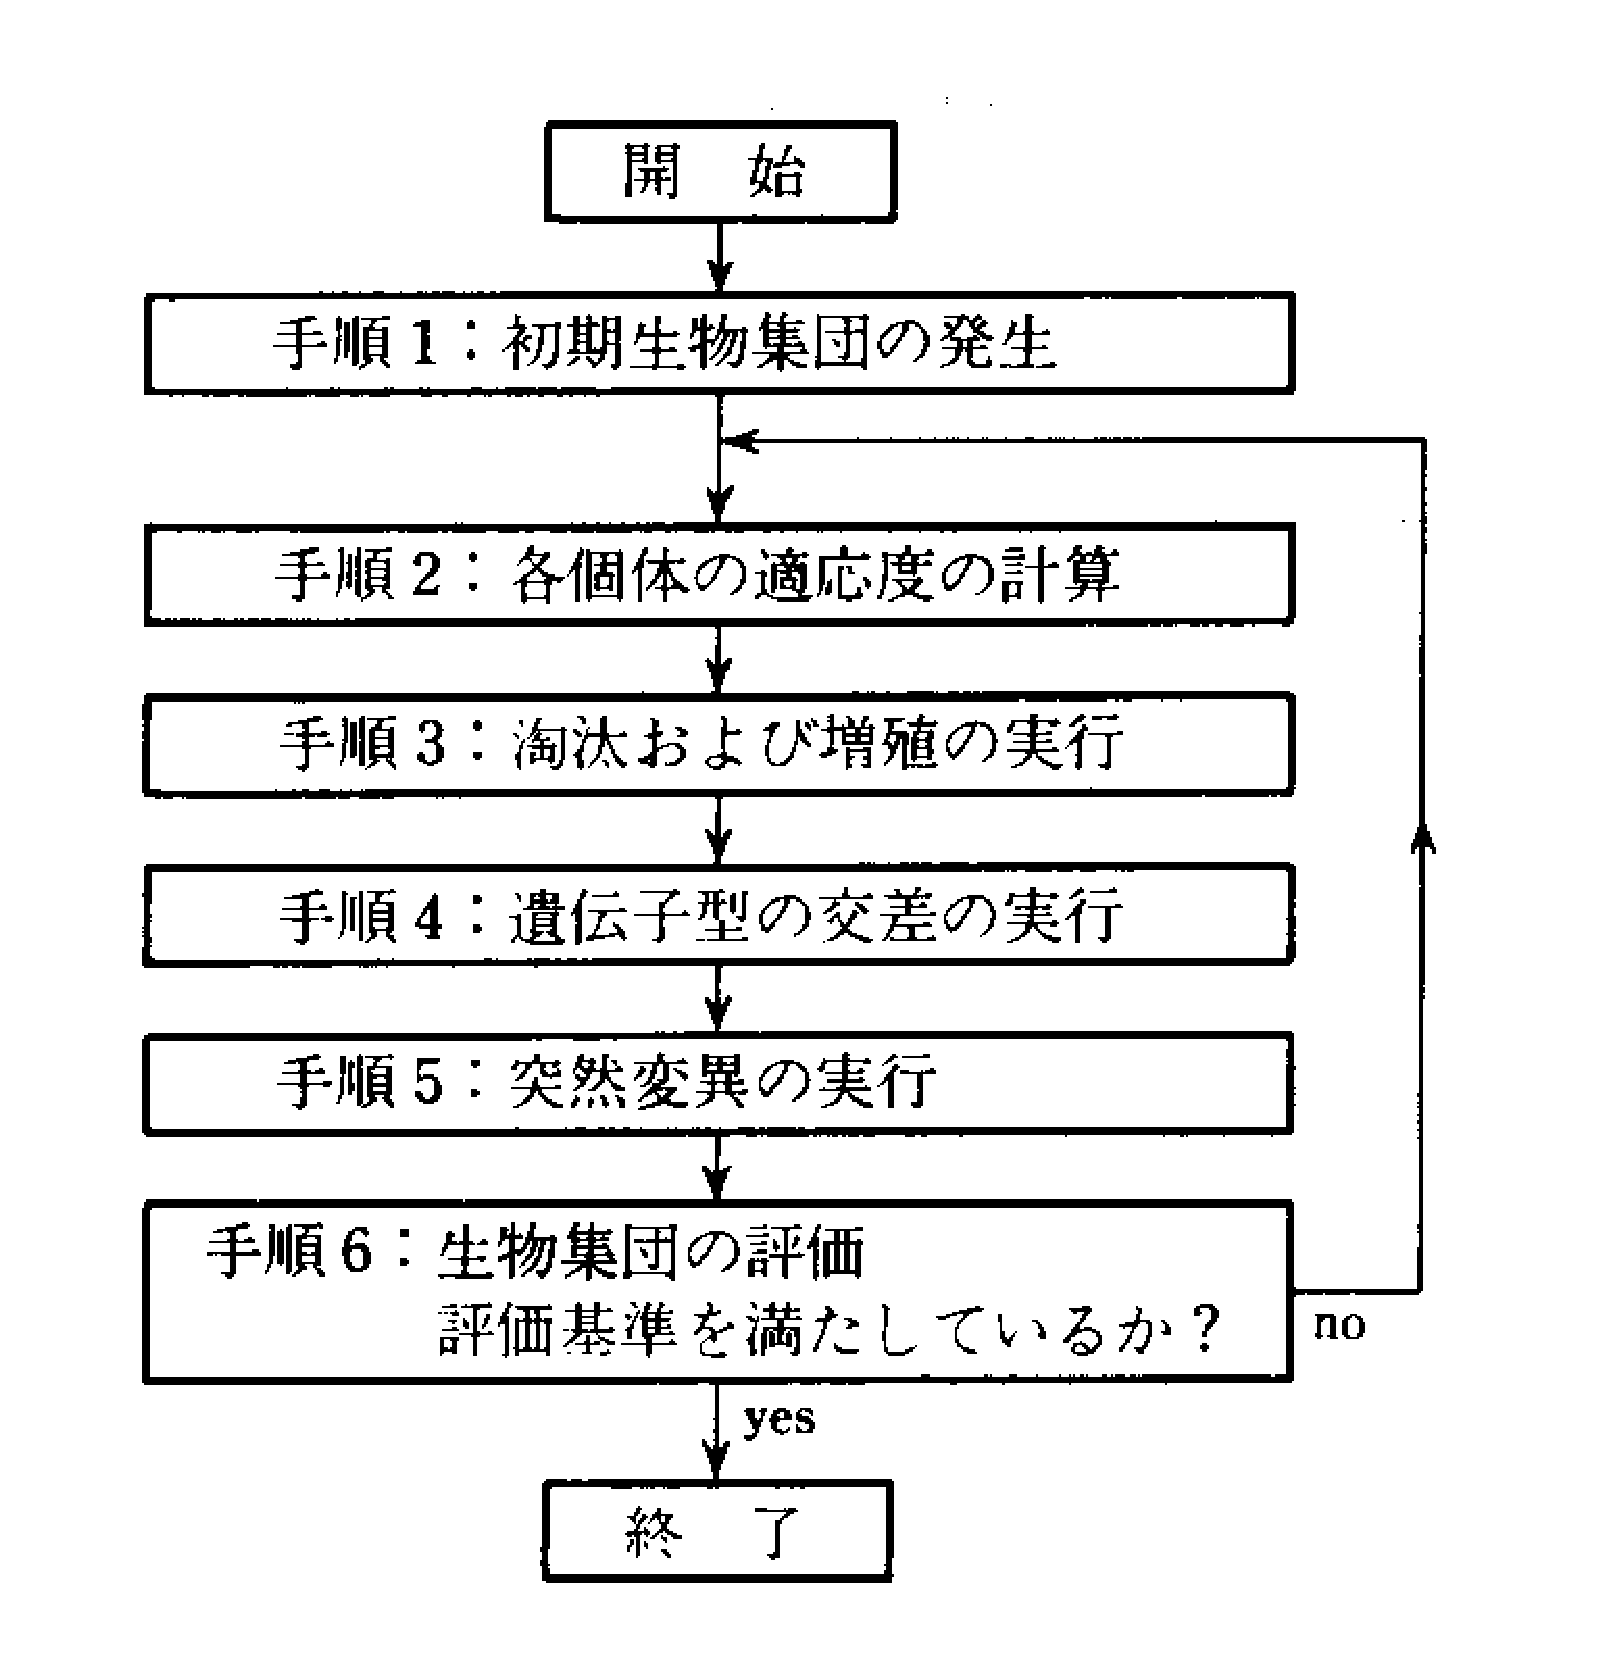
\includegraphics{images/simple_GA.eps}
   }
}
\caption{単純GAの処理手順 \label{SIMPLE_GA}}
\end{center}
\end{figure}

\begin{itemize}
\item[] (1)手順1:初期生物集団の発生
\item[] (2)手順2:各個体の適応度の計算
\item[] (3)手順3:淘汰および増殖の実行
\item[] (4)手順4:遺伝子型の交差の実行
\item[] (5)手順5:突然変異の実行
\item[] (6)手順6:生物集団の評価
\end{itemize}

以上の単純GAをもとに$x^{2}+y^{2}$の最小値を求めるプログラムを
作成しました.

\section{最大・最小におけるGA}

\begin{verbatim}
#include<stdio.h>
#include<math.h>
#include<time.h>
#include<stdlib.h>

#define N      10000    // 個体数
#define CRSS   0.3      // 交差率(Cross over rate)
#define MTTN   0.03     // 突然変異率(Mutation rate)
#define LAST_N 10       // 評価枠(個体数) last number

enum {SLCT, MLTPL};  // SLCT  = SELECT(絶滅)
                     // MLTPL = MULTIPLICATION(増殖)

enum {RANKING, OUT};  // 最終的な評価における項目
                      // 
                      // RANKING : 評価基準満たす
                      // OUT     : 基準を満たさない

typedef struct prm  // (x, y, z) parameters define
{
   double x;
   double y;
   double z;
   int dd_alv;
} OBJ;

double f(double x, double y)
{
   return ( x*x + y*y );
}

void srt(OBJ a[], int first, int last) // QUICK_SORT プログラム(リトルエイディ)
{
   int i , j;
   double cntr;   // cntr = center
   OBJ tmp_obj;

   cntr = a[ (first + last) / 2].z;

   i = first;
   j = last;

   while(1)
   {
       while(a[i].z < cntr)
          i++;

       while(cntr < a[j].z)
          j--;

       if(i >= j)
          break;

       tmp_obj = a[i];
       a[i]    = a[j];
       a[j]    = tmp_obj;

       i++;
       j--;
   }

   if(first < i-1) 
      srt(a, first, i-1);

   if(last > j+1)
      srt(a, j+1, last);
}

void pri(OBJ b[])
{
   int i;

   srt(b, 1, N-1);

   // 評価を満たしたものを表示
   for(i = 1; i <= LAST_N; i++)
   {
         printf("%lf %lf %lf\n\n", b[i].x, b[i].y, b[i].z);
   }
}

void init_xy(OBJ a[])
{
   int i;



   for(i = 1; i < N; i++)
   {
      a[i].x =  drand48();
      a[i].y =  drand48();
      a[i].z = f( a[i].x, a[i].y);
      a[i].dd_alv = MLTPL;  // 生存することを前提にフラグを初期化
   }
}

// 適用度による生存,絶滅
int slt_mlt(OBJ a[])
{
   int i;
   int dist_num = 0;    // 滅んだ数
   double P[N];         // 確率
   double avrg = 0.0;   // 平均値(z)

   for(i = 1; i < N; i++)
   {
      avrg += a[i].z;
   }     
   avrg /= N;

   for(i = 1; i < N; i++)
   {
      P[i] = a[i].z / avrg;

      if(P[i] > avrg)   // 平均値より大きかったら,絶滅
      {
         a[i].dd_alv = SLCT;
         dist_num++;    
      }
   }

   return dist_num;
}

// 交差(crossover)
void crsscvr(OBJ a[])
{
   int i = 1, cnt;
   int fthr, mthr;   // fthr = father, mthr = mother
   double tmp_exch;   // 一時的なデータの格納(temporary exchange)

   cnt = (int) N * CRSS;




   while(i <= cnt)
   {
      fthr = rand() % 71 + 1;
      mthr = rand() % 71 + 1;

      if( MLTPL == a[fthr].dd_alv && MLTPL == a[mthr].dd_alv)
      {
         tmp_exch = a[fthr].x;
         a[fthr].x = a[mthr].x;
         a[mthr].x = tmp_exch;
      }

      i++;
   }
}

// 突然変異(mutation)
void mttn(OBJ a[])
{
   int i = 1, cnt;
   int tgt;        // 突然変異する要素(tgt = target)

   cnt = (int) MTTN * N;

   while(i <= cnt)
   {
      tgt = rand() % 71 + 1;

      if( a[tgt].dd_alv == MLTPL)
      {
         a[tgt].x -= 0.1;
         a[tgt].y -= 0.1;
      }

      i++;
   }
}

// 失ったobejectの分を補う
void add(OBJ a[])
{
   int i;

   for(i = 1; i < N; i++)
   {
      if(a[i].dd_alv == SLCT)
      {
         a[i].x = drand48();
         a[i].y = drand48();
         a[i].z = f( a[i].x, a[i].y );
         a[i].dd_alv == MLTPL;
      }
   }
}

int main(int argc, char *argv[])
{
   int dist_num;                   // 各々の世代の絶滅数
   long ct, gnr = 0;               // 世代交替の回数(gnr = generation)
   OBJ obj[N];                     // オブジェクトの数
   double strt_tm, end_tm;         // 処理計測

   if(argc == 2)
   {
      // 世代数による評価のループ回数
      ct = atoi(argv[1]);
   } else{
      ct = 100;
   }

   // 種の初期化
   srand48(time(NULL)); srand(time(NULL));

   // (x, y)を初期化
   init_xy(obj);


   strt_tm = clock();
   // メイン処理(開始)
   while(1)
   {
      // 1: selection or multiplication
      dist_num = slt_mlt(obj);


      // 2: 遺伝子の交差(crosscover)
      if(dist_num != 0)
         crsscvr(obj);

      // 3: 突然変異(mutation)
      if(gnr % 10 == 10)
         mttn(obj);

      // 4: 評価
      if(gnr >= ct)
         break;


      // 5: 補足
      add(obj);

      gnr++;
   }
   /* メイン処理(終了) */
   end_tm = clock();
   
   /*結果の出力 */
   pri(obj);

   // 所要時間の出力
   printf("所要時間 %f [s]\n", (double) (end_tm - strt_tm) / CLOCKS_PER_SEC);

   return 0;
}
\end{verbatim}

次にこのGAプログラムにMPIで計算するように改良します.

\chapter{MPIによるGA}

1つ前の章の逐次的なプログラムをMPIを使ったプログラムに変更します.
今回用いる並列化はN個のプロセスにおいて, それぞれ逐次的なGAを実行
し, 後にそれぞれの個体をrank 0のプロセスに集め, 評価を行うという
ものです. この並列化は, 任意のプロセス数で扱うことができます.

\begin{verbatim}
#include<stdio.h>
#include<math.h>
#include<time.h>
#include<stdlib.h>
#include "mpi.h"

#define N    10000    // 個体数
#define LAST_N 10     // 評価枠(個体数) last number
                      // ただし, N > LAST_N

#define CRSS 0.3      // 交差率(Cross over rate)
#define MTTN 0.03     // 突然変異率(Mutation rate)

#define ST_N 4        // 構造体の要素のブロック数

enum {SLCT, MLTPL};   // SLCT  = SELECT(絶滅)
                      // MLTPL = MULTIPLICATION(増殖)

enum {RANKING, OUT};  // 最終的な評価における項目
                      // 
                      // RANKING : 評価基準満たす
                      // OUT     : 基準を満たさない

typedef struct prm    // (x, y, z) parameters define
{
   double x;
   double y;
   double z;
   int dd_alv;
} OBJ;

double f(double x, double y)
{
   return ( x*x + y*y );
}

void srt(OBJ a[], int first, int last) // QUICK_SORT プログラム(リトルエイディ)
{
   int i , j;
   double cntr;   // cntr = center
   OBJ tmp_obj;

   cntr = a[ (first + last) / 2].z;

   i = first;
   j = last;

   while(1)
   {
       while(a[i].z < cntr)
          i++;

       while(cntr < a[j].z)
          j--;

       if(i >= j)
          break;

       tmp_obj = a[i];
       a[i]    = a[j];
       a[j]    = tmp_obj;

       i++;
       j--;
   }

   if(first < i-1) 
      srt(a, first, i-1);

   if(last > j+1)
      srt(a, j+1, last);
}

void pri(OBJ b[])
{
   int i;

   // 評価を満たしたものを表示
   for(i = 1; i <= LAST_N; i++)
   {
         printf("%lf %lf %lf\n\n", b[i].x, b[i].y, b[i].z);
   }
}

void init_xy(OBJ a[])
{
   int i;

   for(i = 1; i < N; i++)
   {
      a[i].x =  drand48();
      a[i].y =  drand48();
      a[i].z = f( a[i].x, a[i].y);
      a[i].dd_alv = MLTPL;  // 生存することを前提にフラグを初期化
   }
}

// 適用度による生存,絶滅
int slt_mlt(OBJ a[])
{
   int i;
   int dist_num = 0;    // 滅んだ数
   double P[N];         // 確率
   double avrg = 0.0;   // 平均値(z)

   for(i = 1; i < N; i++)
   {
      avrg += a[i].z;
   }     
   avrg /= N;

   for(i = 1; i < N; i++)
   {
      P[i] = a[i].z / avrg;

      if(P[i] > avrg)   // 平均値より大きかったら,絶滅
      {
         a[i].dd_alv = SLCT;
         dist_num++;    
      }
   }

   return dist_num;
}

// 交差(crossover)
void crsscvr(OBJ a[])
{
   int i = 1, cnt;
   int fthr, mthr;   // fthr = father, mthr = mother
   double tmp_exch;   // 一時的なデータの格納(temporary exchange)

   cnt = (int) N * CRSS;

   while(i <= cnt)
   {
      fthr = rand() % 71 + 1;
      mthr = rand() % 71 + 1;

      if( MLTPL == a[fthr].dd_alv && MLTPL == a[mthr].dd_alv)
      {
         tmp_exch = a[fthr].x;
         a[fthr].x = a[mthr].x;
         a[mthr].x = tmp_exch;
      }

      i++;
   }
}

// 突然変異(mutation)
void mttn(OBJ a[])
{
   int i = 1, cnt;
   int tgt;   // 突然変異する要素(tgt = target)

   cnt = (int) MTTN * N;

   while(i <= cnt)
   {
      tgt = rand() % 71 + 1;

      if( a[tgt].dd_alv == MLTPL)
      {
         a[tgt].x -= 0.1;
         a[tgt].y -= 0.1;
      }

      i++;
   }
}

// 失ったobejectの分を補う
void add(OBJ a[])
{
   int i;

   for(i = 1; i < N; i++)
   {
      if(a[i].dd_alv == SLCT)
      {
         a[i].x = drand48();
         a[i].y = drand48();
         a[i].z = f( a[i].x, a[i].y );
         a[i].dd_alv == MLTPL;
      }
   }
}

int main(int argc, char *argv[])
{
   // For Loop
   int i;

   // MPI Declare
   int myid;                                 // myid = 自分のID 
   int all_nds;                              // all_nds = all nodes (全てのノードの数)            
   int msgt = 99;
   MPI_Status stat;

   int nmln;                                 // プロセッサの名前の長さ
   char prcssr_nm[MPI_MAX_PROCESSOR_NAME];   // プロセッサの名前を格納する 
   double strt_tm, end_tm;                   // 処理の時間計測

   int dist_num;                             // 各々の世代の絶滅数
   long ct, gnr = 0;                         // 世代交替の回数(gnr = generation)

   OBJ s_obj[N], r_obj[N], end_obj[LAST_N];  // s_obj    : send オブジェクト
                                             // r_obj    : receive オブジェクト
                                             // end_obj : 最終的なオブジェクト

   char *rna_recv, *rna_send;       // rna_recv:構造体受信文 rna_send:構造体送信文
   int sz;                                  // size:構造体の送信サイズ
   int pstn;                                 // pstn = position はバッファ中での現在のバイト位置
   int prtnr;                                // 送信相手

   // MPIデータ型の定義(構造体送受信における)
   int blckln[ST_N];                         // blckln = blocklength エントリ数
   MPI_Aint disp[ST_N];                      // disp = displacement はメッセージの先頭からの位置
   MPI_Datatype STR;                         // STR = structure
   MPI_Datatype type[ST_N];                  // type = typelist は各エントリのMPIデータ型

   // MPI Initializations
   MPI_Init(&argc, &argv);
   MPI_Comm_size(MPI_COMM_WORLD, &all_nds);
   MPI_Comm_rank(MPI_COMM_WORLD, &myid);
   MPI_Get_processor_name(prcssr_nm, &nmln);
   //fprintf(stderr, "Process %d on %s\n", myid, prcssr_nm);

   // 送信構造体のタイプの宣言
   type[0] = MPI_DOUBLE;
   type[1] = MPI_DOUBLE;
   type[2] = MPI_DOUBLE;
   type[3] = MPI_INT;
   blckln[0] = 1;
   blckln[1] = 1;
   blckln[2] = 1;
   blckln[3] = 1;
   disp[0] = 0;
   disp[1] = sizeof(double) * 1;
   disp[2] = sizeof(double) * 2;
   disp[3] = sizeof(double) * 3;
   MPI_Type_struct(ST_N, blckln, disp, type, &STR);
   MPI_Type_commit(&STR);

   // 世代数による評価のループ回数
   ct = atoi(argv[1]);

   // 種の初期化
   srand48(time(NULL) + myid); srand(time(NULL) + myid);

   // (x, y)を初期化
   init_xy(s_obj);

   // 時間計測開始
   if(myid == 0)
      strt_tm = MPI_Wtime();

   // メイン処理(開始)
   while(1)
   {
      // 1: selection or multiplication
      dist_num = slt_mlt(s_obj);

      // 2: 遺伝子の交差(crosscover)
      if(dist_num != 0)
         crsscvr(s_obj);

      // 3: 突然変異(mutation)
      if(gnr % 10 == 10)
         mttn(s_obj);

      // 4: 評価
      if(gnr >= ct)
         break;

      // 5: 補足
      add(s_obj);

      gnr++;
   }

   // メイン処理(終了)

   // ソート
   srt(s_obj, 1, N - 1);

   // 構造体の送受信 start
   if(myid != 0){
   // 送受信する構造体のサイズをszに求め代入
   MPI_Pack_size(N, STR, MPI_COMM_WORLD, &sz);

   rna_send = (char *) malloc(sz);

   // 構造体のパック化
   pstn = 0;
   for(i = 0; i < N; i++)
      MPI_Pack(&s_obj[i], 1, STR, rna_send, sz, &pstn, MPI_COMM_WORLD);
   }
  
#if 1
   if(myid != 0)
   {
      MPI_Send(rna_send, pstn, MPI_PACKED, 0, msgt, MPI_COMM_WORLD);
   } else {
      MPI_Recv(r_obj, N, STR, 1, msgt, MPI_COMM_WORLD, &stat);
      pstn = 0;
   }
#endif

#if 0
   MPI_Sendrecv(rna_send, pstn, MPI_PACKED, 0,
                msgt, r_obj, N, STR, 1,
                msgt, MPI_COMM_WORLD, &stat);
#endif

   // myid 0 での処理 それ以外のノードはここで終了
   if(myid == 0)
   {
      // ソート
      //srt(s_obj, 1, 2 * N - 1);

      // MPI時間計測終了
      end_tm = MPI_Wtime();
   
      // 結果の出力
      pri(s_obj);
      printf("\n");
      pri(r_obj);

      // 実行時間出力
      printf("time spended  %f [s]\n", end_tm - strt_tm);
   }

   MPI_Finalize();
}
\end{verbatim}

\begin{thebibliography}{99}
\addcontentsline{toc}{chapter}{\bibname}

\bibitem{pache}
P.パチェコ 訳 秋葉博, MPI並列プログラミング, 培風館,2002

\bibitem{mpi_stan_j}
MPIフォーラム 訳 MPI日本語プロジェクト, MPI:メッセージ
通信インターフェース標準, http://phase.hpcc.jp/phase/mpi-j/ml/, 1996

\bibitem{mpi2_stan_j}
MPIフォーラム 訳 MPI日本語プロジェクト, MPI:メッセージ
通信インターフェースに対する拡張機能, http://phase.hpcc.jp/p
hase/mpi-j/ml/, 1997

\bibitem{mpi2_stan_e}
Message Possing Interface Forum, MPI-2: Extensions to the
Message-Passing Interface, http://www.mpi-forum.org/docs/docs.html,
, 1997

\bibitem{lam_new_inst}
The LAM/MPI Team Open Systems Lab, LAM/MPI Installation Guide
http://www.lam-mpi.org/, 2003

\bibitem{lam_new_user}
The LAM/MPI Team Open Systems Lab, LAM/MPI User's Guide
http://www.lam-mpi.org/, 2003

\bibitem{lam_old}
Ohio Supercomputer Center, MPI Primer Developing With LAM,
http://www.osc.edu/lam.html, 1996

\bibitem{dosisya}
渡邉真也, MPIによる並列プログラミングの基礎,
 http://mikilab.doshis
ha.ac.jp/dia/smpp/cluster2000/PDF/chapter02.pdf, 1997

\bibitem{para_ga}
Rob Davies, An introduction to MPI and Parallel Genetic Algorithm(Cource Notes,
Cardiff HPC Training \& Education Centre

\bibitem{ga}
安居院猛, 長尾智晴, ジェネティックアルゴリズム,
昭晃堂, 1993

\bibitem{ssh}
新山祐介, 春山征吾, OpenSSH セキュリティ管理ガイド,
秀和システム, 2001

\end{thebibliography}

\end{document}
